\documentclass{article}

\input{template}
\usepackage{tikz}

\usepackage[margin=0.5in]{geometry}

\author{Sam Price}
\title{Preview Assignment 1}

\begin{document}
\maketitle

\noindent\textbf{1.} Do any part of Exercise 1.5. (My choice is part A, or $A \union B = A \iff B \subseteq A$)
\begin{proof}
Checking the $A \subseteq B \implies A \union B = A$ direction first, let $A, B$ be sets such that $B \subseteq A$.
As such, when we construct $A \union B = \set{x : x \in A \lor x \in B}$ we find that since $\forall x \in B, x \in A$ that $A \union B = A$.
For the other direction, let $A, B$ be sets such that $A \union B = A$. With this, we see that there exists no $b \in B$ such that $b \notin A$.
This is equivalent to the definition of the subset relation, so we can confidently say then that $B \subseteq A$, and therefore $A \union B = A \iff B \subseteq A$.
\end{proof}

\noindent\textbf{2.} Do both parts of Exercise 1.8 (De Morgan's Laws)
\begin{proof}[Negation of Union]
  Let $x \in (A \union B)'$. Thus, we know $x \notin A \union B \implies x \notin A \land x \notin B$, and therefore that $x \in A' \intersect B'$, since
  $x$ would have to be in both $A'$ and $B'$. As such, we can say that $(A \union B)' \subseteq A' \intersect B'$.
  Now, let $y \in A' \intersect B'$. By our assumption, $y \notin A \land y \notin B$. Thus, we know $y \notin A \union B$ since it is contained within neither set.
  Thus, $y \in (A \union B)'$, and therefore $A' \intersect B' \subseteq (A \union B)' \implies (A \union B)' = A' \intersect B'$.
\end{proof}
\begin{proof}[Negation of Intersection]
  Let $x \in (A \intersect B)'$, which means that $x \notin A \intersect B \implies x \notin A \lor x \notin B$. With $x$ not in at least one of the sets, we know therefore
  that $x \in A' \lor x \in B'$. Thus, $x \in A' \union B'$ and therefore $(A \intersect B)' \subseteq A' \union B'$. Now, let $y \in A' \union B'$.
  We know therefore that $y \notin A \lor y \notin B$, which means it must be in the complement of the intersection as it cannot be in both.
  Thus, we can say that $A' \union B' \subseteq (A \intersect B)'$, and then $A' \union B' = (A \intersect B)'$.
\end{proof}

\noindent\textbf{3.} The function on the left is surjective since each of $\set{a, b, c}$ has an input that ``goes'' to it.
On the other hand, the right function is not because the smiley face does not have any input mapping into it.\\

\noindent\textbf{4.} $f\inv(\set{a}) = \set{1}$, $f\inv(\set{b}) = \set{2, 4}$ and $f\inv(\set{c}) = \set{3}$.\\
For the smiley $s$ (I can't figure out the icons), $f\inv(\set{s}) = \emptyset$.\\

\noindent\textbf{5.} For part (a), the equality holds when $f$ is surjective (assuming nothing else about $B$). Namely, $\nexists b \in B(\nexists x \in X, f(x) = b)$\\
For part (c), equality occurs when $f$ is injective, again assuming nothing malicious about $A$ to deflect from that.
Both can be achieved with weird stuff, like if $f$ was not injective, but having both $x_{1},x_{2}$ that collide in $A$ so that the equality still holds.
If for \textit{any} $A \subseteq X$ and $B \subseteq Y$ (or equivalently, $\forall A \in \mathcal{P}(X)$ and similar), then what was said has no asterisks.\\
Diagram for (b), where $B = \set{3, 41}$ and letting 41 be the best prime number:\\
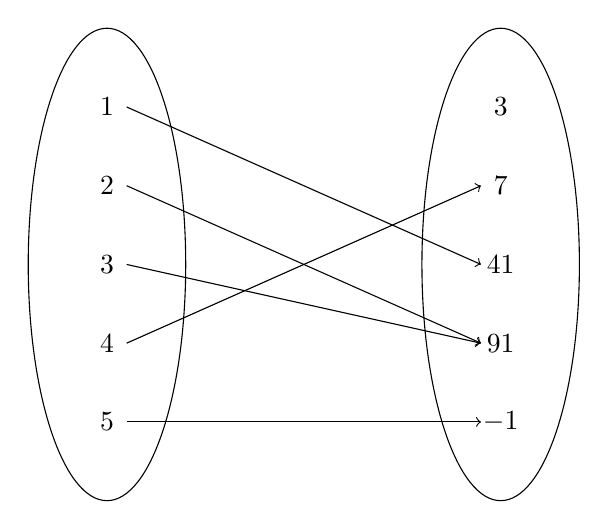
\begin{tikzpicture}
  \draw(0, 0) ellipse (1cm and 3cm);
  \draw(0, 2) node {$1$};
  \draw(0, 1) node {$2$};
  \draw(0, 0) node {$3$};
  \draw(0, -1) node {$4$};
  \draw(0, -2) node {$5$};

  \draw(5, 0) ellipse (1cm and 3cm);
  \draw(5, 2) node {$3$};
  \draw(5, 1) node {$7$};
  \draw(5, 0) node {$41$};
  \draw(5, -1) node {$91$};
  \draw(5, -2) node {$-1$};

  \draw[->] (0.25, 2) -- (4.75, 0);
  \draw[->] (0.25, -1) -- (4.75, 1);
  \draw[->] (0.25, -2) -- (4.75, -2);
  \draw[->] (0.25, 1) -- (4.75, -1);
  \draw[->] (0.25, 0) -- (4.75, -1);
\end{tikzpicture}

Diagram for (d), with $A = \set{1, 2, 4}$:\\
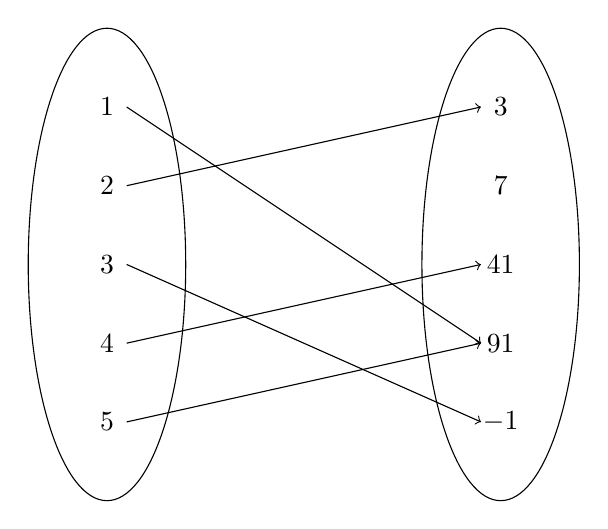
\begin{tikzpicture}
  \draw(0, 0) ellipse (1cm and 3cm);
  \draw(0, 2) node {$1$};
  \draw(0, 1) node {$2$};
  \draw(0, 0) node {$3$};
  \draw(0, -1) node {$4$};
  \draw(0, -2) node {$5$};

  \draw(5, 0) ellipse (1cm and 3cm);
  \draw(5, 2) node {$3$};
  \draw(5, 1) node {$7$};
  \draw(5, 0) node {$41$};
  \draw(5, -1) node {$91$};
  \draw(5, -2) node {$-1$};

  \draw[->] (0.25, 2) -- (4.75, -1);
  \draw[->] (0.25, -2) -- (4.75, -1);
  \draw[->] (0.25, -1) -- (4.75, 0);
  \draw[->] (0.25, 1) -- (4.75, 2);
  \draw[->] (0.25, 0) -- (4.75, -2);
\end{tikzpicture}

\end{document}
